\label{app:analyticalMods}

In this thesis a number of analytical models have been referenced, predominantly the Tsutsui model \cite{Tsutsui:ferrKickLong,Tsutsui:DipoleKicker,Salvant:QuadKicker} and the Mounet model \cite{Mounet:PhDThesis}, representing two finite and infinite parallel plates respectively, and the Zannini mode \cite{Zannini:cCoreFerrite} for C-core ferrite kickers (although valid for any material). In this appendix the methods used in deriving the impedances in these models, known as mode matching, will be briefly discussed.

\section{Tsutsui Model}

\begin{figure}
\begin{center}
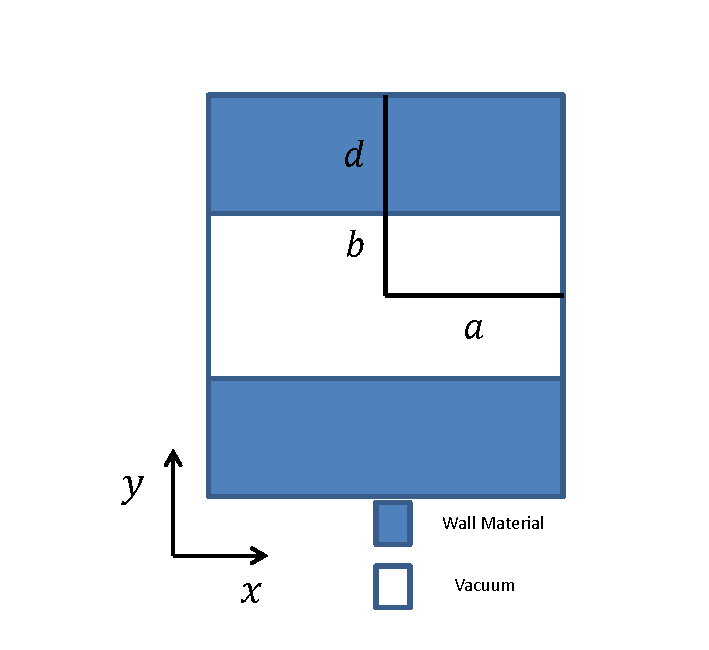
\includegraphics[width=0.6\textwidth]{appendices/figures/tsutsui-geometry.pdf}
\end{center}
\caption{The geometry treated by the Tsutsui model of resistive wall impedance.}
\label{fig:TsutsuiGeo}
\end{figure}

The Tsutsui model of resistive wall impedance defines the impedance for a geometry shown in Fig.~\ref{fig:TsutsuiGeo}, whereby two finite parallel plates of width $2a$, distance $b$ from the centre of the geometry of thickness $d$. For this model derivations for the longitudinal  \cite{Tsutsui:ferrKickLong}, dipolar transverse \cite{Tsutsui:DipoleKicker} and quadrupolar transverse \cite{Salvant:QuadKicker} impedances exist. In addition the longitudinal and dipolar impedance for multi-layered walls has been dervied \cite{Tsutsui:resWallCol}. 

The model works as follows: waveguide modes in each volume (upper wall, vacuum and lower wall) are defined for their respective dimensions, material properties and the source current. In this case image currents are added at $(x,y) = (2na, 0)$ for $n = 0, \pm 1, \pm 2,...$ to account for the perfect electrical boundary at $| x | = a$. These fields are subsequently matched at the boundaries, and the impedance derived from the Fourier transform of the relevant fields ($E_{z}$ for longitudinal impedance, $\mathbf{E}_{\perp}$ and $\mathbf{B}_{\perp}$ for the transverse impedances). 

The impedance per unit length are subsequently given by

\begin{equation}
\frac{Z_{\parallel} \left(f \right)}{L} = j\frac{Z_{0}}{2a} \displaystyle\sum\limits_{n=0} ^{\infty} T_{n}\left(f \right)
\label{eqn:TsutsuiLong}
\end{equation}

for the longitudinal beam coupling impedance,

\begin{equation}
\frac{Z_{x}^{dip}\left(f \right)}{L} = j\frac{Z_{0}}{2a} \displaystyle\sum\limits_{n=0} ^{\infty} \frac{k_{xn}^{2}}{k} T_{n}\left(f \right)
\label{eqn:TsutsuiHorzDip}
\end{equation}

for the horizontal dipolar beam coupling impedance,

\begin{equation}
\frac{Z_{y}^{dip}\left(f \right)}{L} = j\frac{Z_{0}}{2a} \displaystyle\sum\limits_{n=0} ^{\infty} \frac{k_{xn}^{2}}{k} T^{'}_{n}\left(f \right)
\label{eqn:TsutsuiVertDip}
\end{equation}

for the vertical dipolar beam coupling impedance,

\begin{equation}
\frac{Z_{x}^{quad}\left(f \right)}{L} = - j\frac{Z_{0}}{2a} \displaystyle\sum\limits_{n=0} ^{\infty} \frac{k_{xn}^{2}}{k} T_{n}\left(f \right)
\label{eqn:TsutsuiHorzQuad}
\end{equation}

for the horizontal quadrupolar beam coupling impedance, and

\begin{equation}
\frac{Z_{x}^{quad}\left(f \right)}{L} = j\frac{Z_{0}}{2a} \displaystyle\sum\limits_{n=0} ^{\infty} \frac{k_{xn}^{2}}{k} T_{n}\left(f \right)
\label{eqn:TsutsuiVertQuad}
\end{equation}

for the vertical quadrupolar beam coupling impedance, where

\begin{equation}
T_{n}\left(f \right) = \left[ \frac{\frac{k_{xn}}{k\left(f \right)}\left( 1 + \mu_{r}\left(f \right)\epsilon_{r}\left(f \right) \right)sh ch + \frac{k_{yn}\left(f \right)}{k\left(f \right)} \left( \mu_{r}\left(f \right)sh^{2} tn\left(f \right) - \epsilon_{r}\left(f \right) ch^{2} ct\left(f \right) \right)}{\mu_{r}\left(f \right)\epsilon_{r}\left(f \right) -1} - \frac{k\left(f \right)}{k_{xn}}sh ch \right]^{-1},
\end{equation}

\begin{equation}
T^{'}_{n}\left(f \right) = \left[ \frac{\frac{k_{xn}}{k\left(f \right)}\left( 1 + \mu_{r}\left(f \right)\epsilon_{r}\left(f \right) \right)sh ch + \frac{k_{yn}\left(f \right)}{k\left(f \right)} \left( \mu_{r}\left(f \right)ch^{2} tn\left(f \right) - \epsilon_{r}\left(f \right) sh^{2} ct\left(f \right) \right)}{\mu_{r}\left(f \right)\epsilon_{r}\left(f \right) -1} - \frac{k\left(f \right)}{k_{xn}}sh ch \right]^{-1},
\end{equation}

$sh$, $ch$, $tn$, $ct$ are $sinh(K_{xn}b)$, $cosh(k_{xn}b)$, $tan(k_{yn}(b-d))$, $cot(k_{yn}(b-d))$ respectively, $k_{xn} = (2n+1)\pi /(2a)$, $k_{yn}=\sqrt{(\epsilon_{r}\mu_{r} -1)k^{2} - k_{xn}^{2}}$.

\section{Zannini Model}

\begin{figure}
\begin{center}
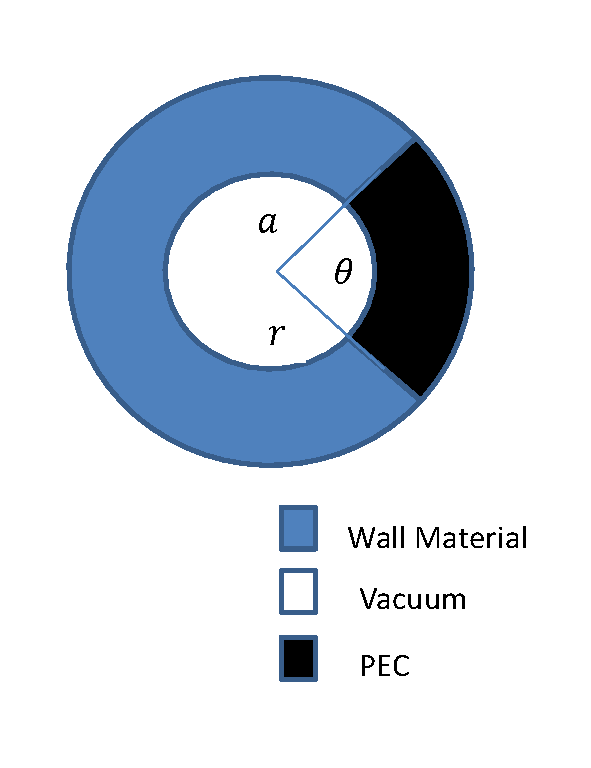
\includegraphics[width=0.6\textwidth]{appendices/figures/zannini-model-geo.pdf}
\end{center}
\caption{The geometry treated by the Zannini model of resistive wall impedance.}
\label{fig:ZanniniGeo}
\end{figure}

The Zannini model is a model of resistive wall impedance designed to model the impedance of a C-core ferrite kicker, shown in Fig.~\ref{fig:ZanniniGeo}. As with the Tsutsui model, the fields are defined for the individual sections of the geometry (vacuum and ferrite) depending on a source current, and then the fields matched at the boundaries between media. In this case, the longitudinal fields of the porpogating TE and TM modes are field, and the transverse fields found by the use of Panofsky-Wenzel theorem.

The derivation in depth is given in \cite{Zannini:cCoreFerrite}.

\section{Mounet Model}

\begin{figure}
\begin{center}
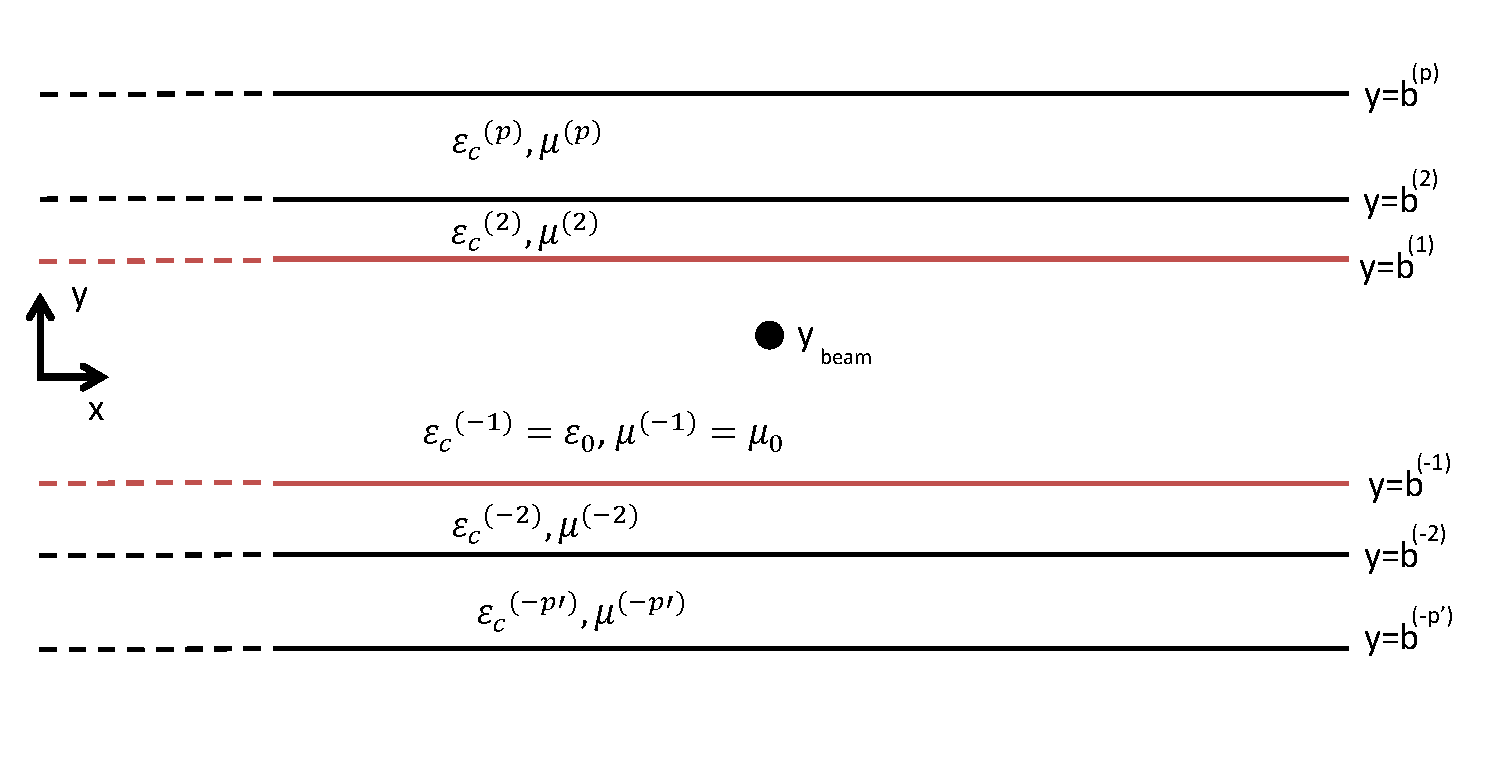
\includegraphics[width=0.6\textwidth]{appendices/figures/mounet-model.pdf}
\end{center}
\caption{The geometry treated by the Mounet model of resistive wall impedance.}
\label{fig:MounetGeo}
\end{figure}

The Mounet model of resistive wall impedance represents the wall impedance of two infinite parallel walls, made of an arbitrary number of layers of material of any well defined (i.e. complex permitivitty/permeability is known for the frequency range of calculation) material which do not necessarily have the same material composition on the top and bottom layers \cite{Mounet:PhDThesis}, for a particle of any relativistic factor $\beta$. This allows the prediction of the longitudinal, horizontal/vertical dipolar, horizontal/vertical quadrupolar and horizontal/vertical constant beam coupling impedances for almost any combination of materials. In particular for low frequency effects on multi-layer devices this is a useful analytical model. 